%
% Tags
%
\subsection{Rótulos dos Itens em Stock}
\subsubsection{Requisitos Legais dos Rótulos}
Segundo o Regulamento (UE) nº1169/2011 \cite{asae:labeling} os rótulos devem conter a seguinte lista de informação:
\begin{itemize}
    \item Denominação da venda;
    \item Listas de ingredientes;
    \item Quantidades de ingredientes ou das categorias de ingredientes;
    \item Quantidade líquida;
    \item Data de durabilidade mínima (DDM)/ Data limite de consumo (DLM);
    \item Condições especiais de conservação e utilização;
    \item Nome ou firma e endereço fabricante, do acondicionador ou do vendedor;
    \item País de origem ou de proveniência;
    \item Instruções de utilização;
    \item Referência ao teor alcoométrico volúmico adquirido.
\end{itemize}

\subsubsection{Rótulos Tradicionais \textit{vs} Rótulos Digitais}
Os códigos de barras são amplamente utilizados na identificação de produtos, quer seja dentro da própria organização, quer seja quando a empresa produtora pretende vender os seus produtos no mercado. Neste último caso, a codificação dos produtos, sendo uma obrigação do mercado, segue as normas da organização GS1\footnote[1]{https://www.gs1.org/}, organização responsável pelo sistema de Normas Globais de Identificação e Codificação de bens e serviços mais utilizado no mundo. A GS1 Portugal é a entidade competente geradora e reguladora da atribuição dos códigos de barras em Portugal. É garantido que não existem dois produtos com o mesmo código de barras em circulação quer a nível nacional, quer a nível global. 

São três os componentes relevantes identificados por um código de barras: o país de origem, a empresa fabricante e o produto produzido, ilustrado na Figura~\ref{bar-code-example}, um exemplo proposto.

\begin{figure}[H]
	\centering
	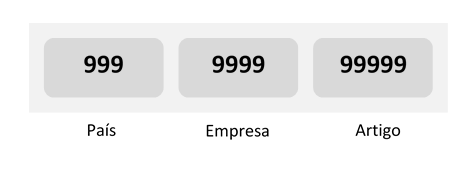
\includegraphics[scale=0.8]{img/codigo_barras_no_background.png}
	\caption{Exemplo proposto de código de barras}
	\label{bar-code-example}
\end{figure}

A gestão de stocks do sistema Smart Stocks necessita de saber o nome do produto, a marca, a variedade, o segmento, a data de validade, os alergénios, a quantidade e, opcionalmente, as condições de conservação. Logo, a informação presente nos códigos de barras é insuficiente para o correto funcionamento do sistema. Como tal, existiu a necessidade de encontrar uma nova abordagem que solucionasse o problema. Uma solução possível passa pela utilização de um leitor de imagens ou de objetos 3D, capaz de ler a informação presente no rótulo tradicional. No entanto, uma outra hipótese é a utilização de rótulos digitais, por exemplo, recorrendo a \textit{tags} \acrfull{nfc} \cite{nfcforum:nfc} ou \acrfull{rfid} \cite{rfidinc:rfid}. 
Como os produtos avulsos têm de ser rotulados, decidiu-se usar \textit{tags} programáveis por \textit{smartphones}. Este processo torna-se prático e acessível a muitos. Ora, uma vez que esta tecnologia é utilizada para os produtos avulsos e sendo uma das soluções possíveis para os produtos embalados, então, uniformiza-se a automatização utilizando a mesma tecnologia nas duas circunstâncias.

\subsubsection{Comparação entre \textit{Tags} NFC e RFID}
\begin{table}[H]
	\centering
	\caption{Comparação da tecnologia \acrshort{nfc} com a tecnologia \acrshort{rfid}}\vspace{2mm}
	\label{tab-comparacao-nfc-vs-rfid}
	\resizebox{\textwidth}{!}{%
		\begin{tabular}{m{6cm}|C{3cm}|C{3cm}}
			
			\textbf{} & \textbf{\acrshort{nfc}} & \textbf{\acrshort{rfid}} \\
			\hline Gama de frequência & 13,56MHz & 125kHz - 960MHz \\
			\hline Comunicação & Unidirecional ou bidirecional (P2P) & Unidirecional \\
			\hline Distância & até 5cm & até 100m \\
			\hline Componentes & Leitor \acrshort{nfc} e \textit{tag} \acrshort{nfc} & Leitor \acrshort{rfid}, \textit{tag} \acrshort{rfid} e uma antena \\
			\hline Suporte em \textit{smartphones} & Na maioria dos \textit{smartphones} & Não \\
			\hline Ativo/Passivo & Passivo, ativado na presença de um leitor \acrshort{nfc} & Passivo, ativado na presença de um leitor \acrshort{rfid} e Ativo, a \textit{tag} tem uma fonte de energia própria \\
			\hline Uso aplicacional & Propriedade desenvolvidas para pagamentos móveis seguros & Usado globalmente para gestão de stocks, manipulação de bagagem no aeroporto, identificação de gado entre outros \\
			\hline Capacidade das \textit{tags} & 64 Bytes até 1024 Bytes & 96 Bits até 512 Bits ou até 4k ou 8k Bytes \\
			
		\end{tabular}
	}
\end{table}

Conforme se pode observar na Tabela \ref{tab-comparacao-nfc-vs-rfid}, a comunicação com as \textit{tags} \acrshort{nfc} pode ser bidirecional o que torna mais fácil e intuitiva a transmissão entre telemóveis e \textit{tags} \acrshort{nfc}. Desta forma, optou-se pela utilização de \textit{tags} \acrshort{nfc} para os produtos avulsos em que é preciso usar o telemóvel para as programar, e, atualmente, os telemóveis só têm suporte para a tecnologia \acrshort{nfc}. Assim os locais de armazenamento têm obrigatoriamente de dispor de leitor de \textit{tags} \acrshort{nfc}. Contudo, se os embaladores decidirem utilizar \acrshort{rfid}, o hardware pode também ter leitor \acrshort{rfid}. O levantamento de requisitos feito, juntamente com a dimensão dos campos da base de dados, e sabendo que o formato utilizado na escrita das \textit{tags} é \acrfull{csv} \cite{RFC4180:csv}, estimou-se que a capacidade de armazenamento mínima das \textit{tags} é aproximadamente 324 Bytes.
